\documentclass[11pt,letterpaper]{article}
\usepackage[utf8]{inputenc}
\usepackage[left=1in,right=1in,top=1in,bottom=1in]{geometry}
\usepackage{amsfonts,amsmath}
\usepackage{graphicx,float}
\usepackage{csquotes}
% -----------------------------------
\usepackage{hyperref}
\hypersetup{%
  colorlinks=true,
  linkcolor=blue,
  citecolor=blue,
  urlcolor=blue,
  linkbordercolor={0 0 1}
}
% -----------------------------------
\usepackage[style=authoryear-icomp,backend=biber]{biblatex}
\addbibresource{citation.bib}
% -----------------------------------
\usepackage{fancyhdr}
\newcommand\course{MATH-UA.0263\\Partial Differential Equations}
\newcommand\hwnumber{9}                  % <-- homework number
\newcommand\NetIDa{Ryan Sh\`iji\'e D\`u} 
\newcommand\NetIDb{April 6th, 2023}
\pagestyle{fancyplain}
\headheight 35pt
\lhead{\NetIDa\\\NetIDb}
\chead{\textbf{\Large Worksheet \hwnumber}}
\rhead{\course}
\lfoot{}
\cfoot{}
\rfoot{\small\thepage}
\headsep 1.5em
% -----------------------------------
\usepackage{titlesec}
\renewcommand\thesubsection{(\arabic{section}.\alph{subsection})}
\titleformat{\subsection}[runin]
        {\normalfont\bfseries}
        {\thesubsection}% the label and number
        {0.5em}% space between label/number and subsection title
        {}% formatting commands applied just to subsection title
        []% punctuation or other commands following subsection title
% -----------------------------------
\setlength{\parindent}{0.0in}
\setlength{\parskip}{0.1in}
% -----------------------------------
\newcommand{\de}{\mathrm{d}}
\newcommand{\DD}{\mathrm{D}}
\newcommand{\pe}{\partial}
\newcommand{\mcal}{\mathcal}
%\newcommand{\pdx}{\left|\frac{\partial}{\partial_x}\right|}

\newcommand{\dsp}{\displaystyle}

\newcommand{\norm}[1]{\left\Vert #1 \right\Vert}
%\newcommand{\mean}[1]{\left\langle #1 \right\rangle}
\newcommand{\mean}[1]{\overline{#1}}
\newcommand{\inner}[2]{\left\langle #1,#2\right\rangle}

\newcommand{\ve}[1]{\boldsymbol{#1}}

\newcommand{\thus}{\Rightarrow \quad }
\newcommand{\fff}{\iff\quad}
\newcommand{\qdt}[1]{\quad \mbox{#1} \quad}

\renewcommand{\Re}{\mathrm{Re}}
\renewcommand{\Im}{\mathrm{Im}}
\newcommand{\E}{\mathbb{E}}
\newcommand{\lap} {\nabla^2}
\renewcommand{\div}{\nabla\cdot}

\newcommand{\csch}{\text{csch}}
\newcommand{\sech}{\text{sech}}


\newcommand{\hot}{\text{h.o.t.}}

\newcommand{\ssp}{\left.\qquad\right.}

\newcommand{\var}{\text{var}}
\newcommand{\cov}{\text{cov}}


\begin{document}

\section{Alternative formula for Fourier transform}
In the HW you have one definition of the Fourier transform and its associated inversion formula:
\begin{align}
    &\hat f(\xi) = \int f(x)e^{-i\xi x} \;\de x,\\
    &f(x) = \int \hat f(\xi)e^{+i\xi x} \;\de \xi \cdot\frac{1}{2\pi}.
\end{align}
An alternative formula that absorbs the $2\pi$ factor into the Fourier kernal is:
\begin{align}
    &\hat f(\xi ) = \int f(x)e^{-2\pi i\xi x} \;\de x,\\
    &f(x) = \int \hat f(\xi)e^{+2\pi i \xi x} \;\de \xi \label{eq:Four_inv}.
\end{align}
Show that the second version is also valid. I would use the second version in this note.

\section{Some example dispersion relations}
\subsection{}
The Korteweg–De Vries equation is a nonlinear, dispersive PDE that models waves on shallow water surfaces
\begin{align}
    u_t+u_{xxx}-6uu_x = 0.
\end{align}
It is clear that zero is a solution. Linearize the equation around the zero solution. That is, assume the amplitude of the solution is small. We get
\begin{align}
    w_t+w_{xxx} = 0.
\end{align}
What is the dispersion relation? What is the phase velocity and group velocity?

\subsection{}
Kuramoto-Sivashinsky equation or the flame equation model a flame front. 
\begin{align}
    u_t+u_{xx}+u_{xxxx}+\frac{1}{2}u_x^2 = 0.
\end{align}
It is known for its chaotic behavior. Again linearize around the zero solution to get the linear PDE
\begin{align}
    w_t+w_{xxxx}+w_{xx} = 0.
\end{align}
Calculate the same three quantities.

\subsection{}
We study the sine-Gordon equation
\begin{align}
    u_{tt} = c^2u_{xx}-\sin(u).
\end{align}
Linearize around the zero solution. Calculate the same three quantities.

\section{Numerical diffusion and dispersion}
[From \S 10.9 of \cite{LeVeque_07}] We will study finite difference scheme for the advection equation
\begin{align}
    u_t+au_x = 0.
\end{align}
We assume $a>0$ and $a=O(1)$. 

\subsection{}
We could use the upwinding scheme
\begin{align}
    U^{n+1}_j = U^n_j-\frac{a\Delta t}{\Delta x}\left( U^n_j-U^n_{j-1} \right).
\end{align}
Show that the upwinding scheme is a consistent approximation of the PDE using Taylor expansion. 

\subsection{}
Take a function $v(x,t)$ that satisfy the upwinding scheme exactly:
\begin{align}
    v(x,t+\Delta t)=v(x,t)-\frac{a\Delta t}{\Delta x}\left[v(x,t)-v(x-\Delta x,t)\right].
\end{align}
Show that up to an $O(\Delta t^2)$ approximation the PDE that $v$ satisfies is
\begin{align}
    v_t+av_x = \frac{1}{2}a\Delta x\left(1-\frac{a\Delta t}{\Delta x}\right)v_{xx}.
\end{align}
This is called the modified equation of the upwinding scheme.

Therefore the numerical error when we use the upwinding scheme is diffusive in nature.

\begin{figure}[H]
    \centering
    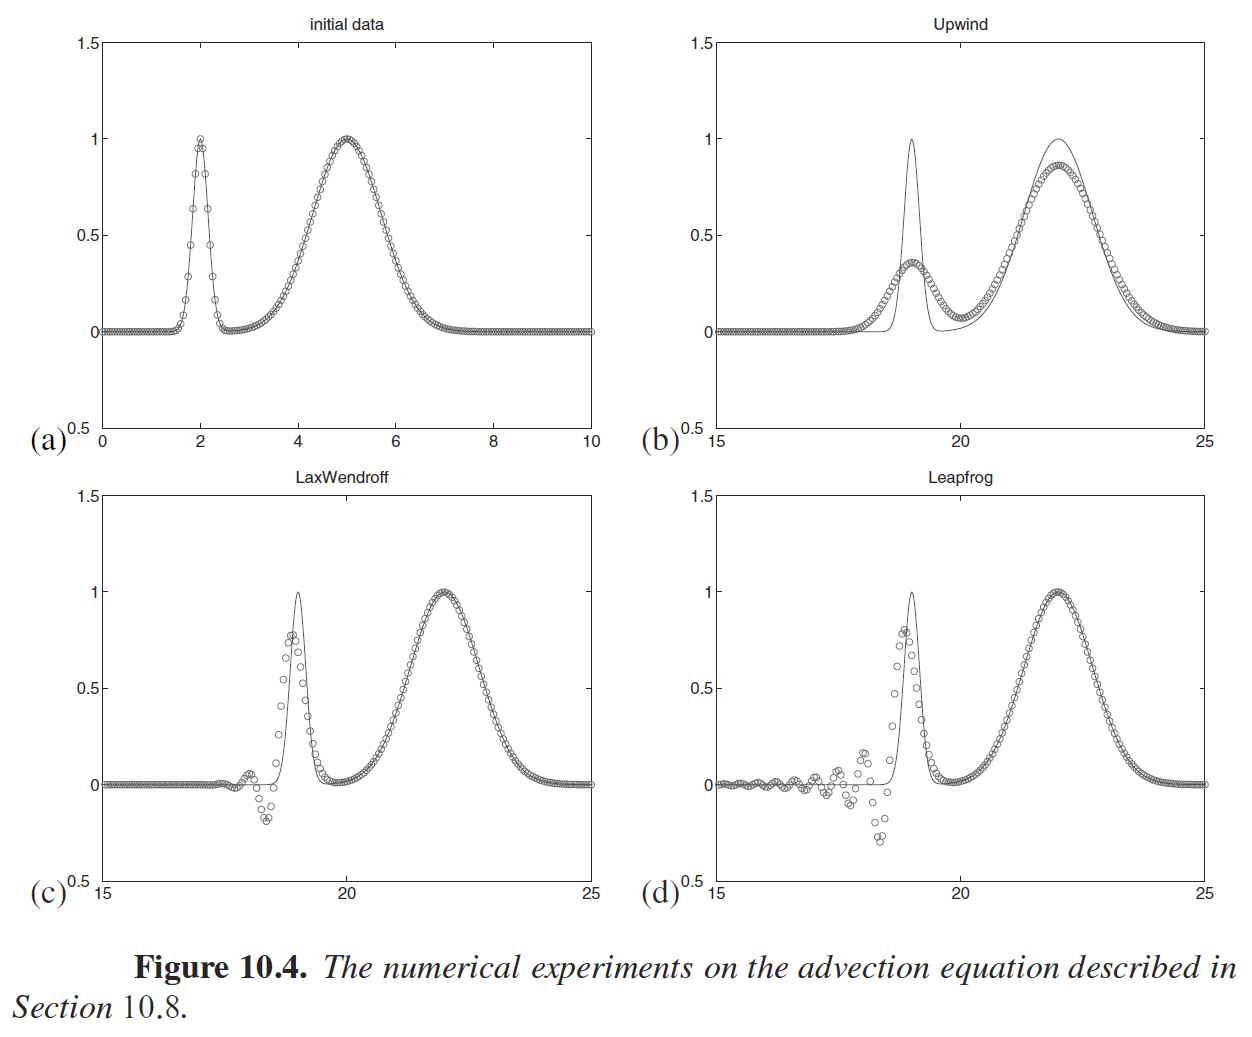
\includegraphics[width=0.8\textwidth]{figs/num_dispers}
\end{figure}

\subsection{}
A better approximation to the advection equation gives the Lax-Wendroff scheme:
\begin{align}
    U^{n+1}_j = U^n_j-\frac{a\Delta t}{2\Delta x}\left( U^n_{j+1}-U^n_{j-1} \right)+\frac{a^2 \Delta t^2}{2\Delta x^2}\left(U^n_{j+1}-2U^n_{j}+U^n_{j-1}\right).
\end{align}
A rather long calculation\footnote{see \url{https://guillod.org/teaching/m2-b004/TD2-solution.pdf}} gives the modified equation of the Lax-Wendroff scheme:
\begin{align}
    v_t+av_x +\frac{1}{6}a\Delta x^2\left(1-\left(\frac{a\Delta t}{\Delta x}\right)^2\right)v_{xxx} = 0.
\end{align}
Calculate the dispersion relationship for waves in this PDE. Are the waves dispersive? What is the group velocity? We say that the error for the Lax-Wendroff is dispersive in nature. 

For stability, we require the ratio
\begin{align}
    \frac{a\Delta t}{\Delta x}<1.
\end{align}
Compare the group velocity to the advection velocity. Use this to explain the trailing wavy error in the above figure for Lax-Wendroff. 

\subsection{}
The above plot also show the Leapfrog scheme, which also has dispersive error. Another scheme is the Beam-Warming scheme. We see from the figure below that its error is also dispersive, but the error lead the solution. You could do the same calculation and see that $c_g>a$. 
\begin{figure}[H]
    \centering
    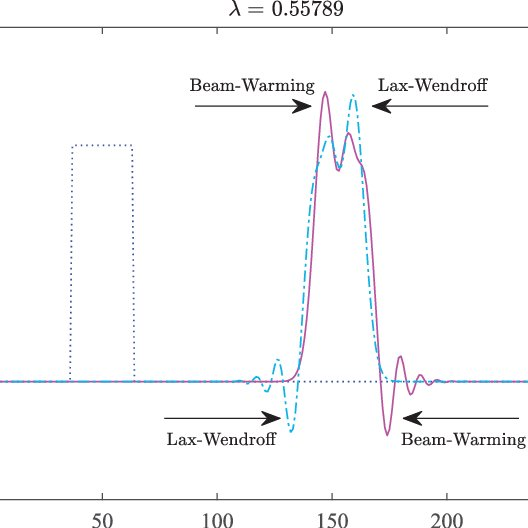
\includegraphics[width=0.6\textwidth]{figs/beamwarming}
\end{figure}


\section{Riemann-Lebesgue Lemma}
The mathematical theorem that is behind the method of stationary phase is the Riemann-Lebesgue Lemma. 
\begin{displayquote}
    Let $f:\mathbb{R}\to\mathbb{R}$ be a (Lebesgue) integrable function. Then we have
    \begin{align}
        \lim_{\xi\to\infty} \int^\infty_{-\infty} f(x)e^{i\xi x}\;\de x = 0
    \end{align}
\end{displayquote}
Intuitively, as $\xi$ increases the oscillations in the integral increase and become much faster than any variation in $f(x)$; successive oscillations thus cancel and the integral becomes very small.

\subsection{}
Show this result assuming $f(x)$ is the indicator function for some compact set. Extend the result to step functions which is piecewise constant. 

\subsection{}
Compact (Lebesgue) integrable function can be approximated arbitrary well by step functions. That is, for all $\epsilon>0$ there is a step function $\varphi$ such that
\begin{align}
    \left| \int_M f \;\de x - \int_M \varphi \;\de x \right| < \epsilon.
\end{align}
Use this fact to show that the Riemann-Lebesgue Lemma holds for compact (Lebesgue) integrable function.

\subsection{}
Finally, show that Riemann-Lebesgue Lemma holds for any (Lebesgue) integrable function. That is, function such that
\begin{align}
    \int_\mathbb{R} |f|\;\de x < \infty.
\end{align}


\vfill
\printbibliography


\end{document}